\documentclass[11pt]{article}
%\usepackage{graphicx}
\usepackage{booktabs}
\usepackage[backend=bibtex]{biblatex}
%\addbibresource{myBibRefsFile.bib}
%\usepackage[backend=bibtex,style=verbose-trad2]{biblatex}
\bibliography{IT.bib}
\usepackage{float}

%\usepackage[margin=1in]{geometry}
\usepackage{fancyhdr}
%\pagestyle{fancy}
\usepackage{amsmath}
%\usepackage{amssymb}
%\usepackage[table]{xcolor}
\usepackage{bm}
\usepackage{array}
\usepackage{mathtools}
\usepackage{soul,soulutf8}
\usepackage{url,color}
\usepackage{fullpage}
\usepackage[english]{babel}

\usepackage[utf8]{inputenc}
\lhead{STA 4001: Stochastic Processes}
\chead{}
\rhead{\textup{CUHK(SZ) Fall 2018}}


\usepackage{amsmath,amsthm,amssymb}
%\usepackage{extarrows}
%\usepackage{breqn}
\usepackage{mathtools}
\DeclarePairedDelimiter\ceil{\lceil}{\rceil}
\DeclarePairedDelimiter\floor{\lfloor}{\rfloor}
\newcommand{\N}{\mathbb{N}}
\newcommand{\Z}{\mathbb{Z}}
\newcommand{\trans}{^{\mathrm T}}

\newenvironment{theorem}[2][Theorem]{\begin{trivlist}
\item[\hskip \labelsep {\bfseries #1}\hskip \labelsep {\bfseries #2.}]}{\end{trivlist}}
\newenvironment{lemma}[2][Lemma]{\begin{trivlist}
\item[\hskip \labelsep {\bfseries #1}\hskip \labelsep {\bfseries #2.}]}{\end{trivlist}}
\newenvironment{exercise}[2][Exercise]{\begin{trivlist}
\item[\hskip \labelsep {\bfseries #1}\hskip \labelsep {\bfseries #2.}]}{\end{trivlist}}
\newenvironment{reflection}[2][Reflection]{\begin{trivlist}
\item[\hskip \labelsep {\bfseries #1}\hskip \labelsep {\bfseries #2.}]}{\end{trivlist}}
\newenvironment{proposition}[2][Proposition]{\begin{trivlist}
\item[\hskip \labelsep {\bfseries #1}\hskip \labelsep {\bfseries #2.}]}{\end{trivlist}}
\newenvironment{corollary}[2][Corollary]{\begin{trivlist}
\item[\hskip \labelsep {\bfseries #1}\hskip \labelsep {\bfseries #2.}]}{\end{trivlist}}
\DeclareMathOperator{\tr}{tr}
\DeclareMathOperator{\rank}{rank}
\DeclareMathOperator{\Span}{span}
\DeclareMathOperator{\row}{row}
\DeclareMathOperator{\col}{col}
\DeclareMathOperator{\range}{range}
\DeclareMathOperator{\Null}{Null}
\DeclarePairedDelimiterX{\inp}[2]{\langle}{\rangle}{#1, #2}
\DeclareMathOperator{\Proj}{Proj}
\newcommand{\diff}{\,\mathrm{d}}
\DeclareMathOperator{\trace}{trace}
\newcommand{\Her}{^{\mathrm H}}
\DeclareMathOperator{\diag}{diag}
\newcommand{\Var}{\mathrm{Var}}
%\usepackage{listings}
%\usepackage{color} %red, green, blue, yellow, cyan, magenta, black, white
%\definecolor{mygreen}{RGB}{28,172,0} % color values Red, Green, Blue
%\definecolor{mylilas}{RGB}{170,55,241}
%
%
%\lstset{language=Matlab,%
%    %basicstyle=\color{red},
%    breaklines=true,%
%    morekeywords={matlab2tikz},
%    keywordstyle=\color{blue},%
%    morekeywords=[2]{1}, keywordstyle=[2]{\color{black}},
%    identifierstyle=\color{black},%
%    stringstyle=\color{mylilas},
%    commentstyle=\color{mygreen},%
%    showstringspaces=false,%without this there will be a symbol in the places where there is a space
%    numbers=left,%
%    numberstyle={\tiny \color{black}},% size of the numbers
%    numbersep=9pt, % this defines how far the numbers are from the text
%    emph=[1]{for,end,break},emphstyle=[1]\color{red}, %some words to emphasise
%    %emph=[2]{word1,word2}, emphstyle=[2]{style},    
%}
\usepackage{listings}
\RequirePackage{listings}
\RequirePackage{xcolor}
\definecolor{dkgreen}{rgb}{0,0.6,0}
\definecolor{gray}{rgb}{0.5,0.5,0.5}
\definecolor{mauve}{rgb}{0.58,0,0.82}
\lstset{
  frame=tb,
  aboveskip=3mm,
  belowskip=3mm,
  showstringspaces=false,
  columns=flexible,
  framerule=1pt,
  rulecolor=\color{gray!35},
  backgroundcolor=\color{gray!5},
  basicstyle={\small\ttfamily},
  numbers=none,
  numberstyle=\tiny\color{gray},
  keywordstyle=\color{blue},
  commentstyle=\color{dkgreen},
  stringstyle=\color{mauve},
  breaklines=true,
  breakatwhitespace=true,
  tabsize=3,
}

\newcommand{\degree}{\ensuremath{^\circ}}
\begin{document}
\title{\bfseries\upshape{Solution to Assignment 5}}%replace X with the appropriate number
\author{\textit{I will appreciate it if you could give me some advice on my assignment!}} %if necessary, replace with your course title
\maketitle
\section*{phd exercise}
\begin{enumerate}
\item
Given the standard form of LP problem
\[
\begin{array}{ll}
\min&\bm c\trans\bm x\\
\mbox{such that}&\bm{Ax}=\bm b\\
&\bm x\ge0
\end{array}
\]
with $\bm A\in\mathbb{R}^{m\times n}$, $m<n$, $\bm b\in\mathbb{R}^m$ and $\bm c\in\mathbb{R}^n$, we apply the pdipm to solve this problem, i.e., solve the linear system (\ref{Eq:1}):
\begin{equation}
\begin{array}{ll}
F(\bm x,\bm y,\bm z)=\begin{pmatrix}
\bm A\trans\bm y+\bm z-\bm c\\
\bm{Ax}-\bm b\\
\bm x\circ\bm z
\end{pmatrix}=\bm0,
&
(\bm x,\bm z)\ge0.
\end{array},\label{Eq:1}
\end{equation}
which is also the \emph{optimality conditions} of the standard form LP. Prove that the \emph{Jacobian matrix} $F'(\bm x,\bm y,\bm z)$ is non-singular if $(\bm x,\bm z)>0$ and $\bm A$ has the \emph{full row rank}.
\begin{proof}
As have done in last assignment, we obtain:
\[
F'(\bm x,\bm y,\bm z):=\bm Y=\begin{pmatrix}
\bm0&\bm A\trans&\bm I\\
\bm A&\bm0&\bm0\\
\bm Z&\bm 0&\bm X
\end{pmatrix}_{(n+m+n)\times(n+m+n)}
\]
with $\bm Z=\diag(z_1,\dots,z_n)$ and $X=\diag(x_1,\dots,x_n)$. Given the condition that $\rank(\bm A)=m<n$ and $(\bm x,\bm z)>0$, it suffices to show that the null space matrix $\bm Y$ has only trivial solution, i.e., $\mathcal{N}(\bm Y)=\{\bm0\}$. Given any $(\bm u,\bm v,\bm w)\in\mathbb{R}^n\times\mathbb{R}^m\times\mathbb{R}^n$ in the null space $\mathcal{N}(\bm Y)$, it suffices to show $(\bm u,\bm v,\bm w)=(\bm0,\bm0,\bm0)$. From $\bm Y(\bm u,\bm v,\bm w)=(\bm0,\bm0,\bm0)$ we derive:
\begin{subequations}
\begin{align}
\bm A\trans\bm v+\bm w&=\bm0\label{Eq:2:1}\\
\bm A\bm u&=\bm0\label{Eq:2:2}\\
\bm Z\bm u+\bm X\bm w&=\bm0\label{Eq:2:3}
\end{align}
\end{subequations}
\begin{itemize}
\item
Left-multiplying (\ref{Eq:2:1}) with $\bm u\trans$ and noting (\ref{Eq:2:2}), we derive:
\begin{equation}
\bm u\trans\bm w=\bm0\label{Eq:3}
\end{equation}

We re-write (\ref{Eq:2:3}) as:
\begin{subequations}
\begin{align}
\bm u+\bm Z^{-1}\bm X\bm w&=0\\
\bm w+\bm X^{-1}\bm Z\bm u&=0
\end{align}
\end{subequations}

Combining with (\ref{Eq:3}), equialently we have
\begin{subequations}
\begin{align}
\bm w\trans\bm Z^{-1}\bm X\bm w&=0\\
\bm u\trans\bm X^{-1}\bm Z\bm u&=0
\end{align}
\end{subequations}

Note that $\bm Z,\bm X\succ0$, i.e., $\bm Z^{-1}\bm X,\bm X^{-1}\bm Z\succ0$, which implies $\bm w=\bm u=\bm0$.
\item
Finally, consider that $\bm w=\bm0$ and (\ref{Eq:2:1}), we derive $\bm A\trans\bm v=\bm0$. Since $\rank(\bm A\trans)=m$, i.e., columns of $\bm A\trans$ are linearly independent, we derive $\bm v=\bm0$.
\end{itemize}
The proof is complete. 
\end{proof}

\item
Let $x^*$ be a faesible point that is \emph{regular} and together with some $\lambda^*$ satisfies the first and second order necessary conditions:
\begin{subequations}
\begin{align}
\nabla f(x^*)+\sum_{i=1}^m\lambda_i^*\nabla h_i(x)&=0\Longleftrightarrow
\nabla_x L(x^*,\lambda^*)=0
\\
y\trans\left[\nabla^2 f(x^*)+\sum_{i=1}^m\lambda_i^*\nabla^2 h_i(x)\right]y&\ge0
\Longleftrightarrow y\trans
\nabla^2_{xx} L(x^*,\lambda^*)y\ge0,
\quad
\mbox{for all $y\ne0$ with $\inp{\nabla h(x^*)}{y}=\bm0$}
\label{Eq:6:b}
\end{align}
\end{subequations}
Show that $x^*$ and $\lambda^*$ satisfy the sufficient conditions 
\begin{subequations}
\begin{align}
\nabla_xL(x^*,\lambda^*)&=0,\qquad
\nabla_\lambda L(x^*,\lambda^*)=0,\\
y\trans\nabla^2_{xx}L(x^*,\lambda^*)y&>0,\qquad
\mbox{for all $y\ne0$ with $\inp{\nabla h(x^*)}{y}=\bm0$}\label{Eq:7:2}
\end{align}
\end{subequations}
if and only if the matrix
\[\bm R=
\begin{pmatrix}
\nabla_{xx}^2L(x^*,\lambda^*)&\nabla h(x^*)\\
\nabla\trans h(x^*)&0
\end{pmatrix}
\]
is non-singular.
\begin{proof}
Necessity. To show the forward assertion, assume $\bm R$ is singular, i.e., there exists nonzero vector $(w,v)$ that is in the null space of $\bm R$, i.e.,
\begin{subequations}
\begin{align}
\nabla_{xx}^2L(x^*,\lambda^*)w+\nabla h(x^*)v&=0\label{Eq:8:1}\\
\inp{\nabla h(x^*)}{w}&=0\label{Eq:8:2}
\end{align}
\end{subequations}
\begin{itemize}
\item
Left-multiplying (\ref{Eq:8:1}) with $w\trans$, and consider (\ref{Eq:8:2}), we derive:
\begin{equation}
w\trans\nabla_{xx}^2L(x^*,\lambda^*)w=0
\end{equation}
As $\inp{\nabla h(x^*)}{w}=0$, consider (\ref{Eq:7:2}), we derive $w=0$. Substituting $w$ into (\ref{Eq:8:1}),we derive $v=0$, since $\nabla h_1(x^*),\dots,\nabla h_m(x^*)$ is linearly independent. Thus we derive a contradiction. Hence, $\bm R$ must be non-singular.
which follows that $v=0$.
\end{itemize}
Sufficiency. Assume that there exists $\bar y\ne0$ such that $\inp{\nabla h(x^*)}{\bar y}=0$ but $\bar{y}\trans\nabla^2_{xx}L(x^*,\lambda^*)\bar y=0$ (From (\ref{Eq:6:b}), note that $\bar{y}\trans\nabla^2_{xx}L(x^*,\lambda^*)\bar y\ge0$ for any $\bar y\ne0$ such that $\inp{\nabla h(x^*)}{\bar y}=0$). Thus $\bar y$ is essentially the local minimum for the optimization problem
\begin{equation}\label{Eq:10}
\begin{array}{ll}
\min&y\trans\nabla^2_{xx}L(x^*,\lambda^*)y\\
\mbox{such that}&\inp{\nabla h(x^*)}{y}=0
\end{array}
\end{equation}
Consider the Lagrange function $G(y,\mu)=y\trans\nabla^2_{xx}L(x^*,\lambda^*)y+\mu\inp{\nabla h(x^*)}{y}$, applying the first order necessary condition for constraint problem, we have
\[
\nabla_yG(\bar y,\bar \mu)
=
2\nabla^2_{xx}L(x^*,\lambda^*)\bar y+\bar\mu^*\nabla h(x^*)=0.
\]
Combining with the condition $\inp{\nabla h(x^*)}{\bar y}=0$, we obtain a matrix-form system:
\[
\begin{pmatrix}
\nabla_{xx}^2L(x^*,\lambda^*)&\nabla h(x^*)\\
\nabla\trans h(x^*)&0
\end{pmatrix}\begin{pmatrix}
2\bar y\\\bar\mu
\end{pmatrix}=\begin{pmatrix}
0\\0
\end{pmatrix}
\]
Therefore, $(2\bar y,\bar\mu)\in\mathcal{N})(\bm R)$ but $\bar y\ne0$, i.e., the null space of $\bm R$ contains a non-trivial solution, which is a contradiction.

The proof is complete.






\end{proof}

\item
Let $x^*$ be a faesible point that is \emph{regular} and together with some $\lambda^*$ satisfies the first and second order necessary conditions:
\begin{subequations}
\begin{align}
\nabla_xL(x^*,\lambda^*)&=0,\qquad
\nabla_\lambda L(x^*,\lambda^*)=0,\\
y\trans\nabla^2_{xx}L(x^*,\lambda^*)y&>0,\qquad
\mbox{for all $y\ne0$ with $\inp{\nabla h(x^*)}{y}=\bm0$}\label{Eq:8:2}
\end{align}
\end{subequations}
then for some u and corresponding $\lambda(u)$ in the ppen sphere $S$ centered at $u=0$, for every scalar $c$ for which the matrix
\begin{equation}\label{Eq:12}
A_c(u)=\nabla^2_{xx}L(x(u),\lambda(u))+c\nabla h(x(u))\nabla\trans h(x(u))
\end{equation}
is invertible, we have
\begin{equation}\label{Eq:13}
\nabla^2 p(u) = \left(\nabla\trans h(x(u))A_c(u)^{-1}\nabla h(x(u))\right)^{-1}-cI
\end{equation}
\begin{proof}
From the sensitivity theorem, we have
\begin{subequations}
\begin{align}
\nabla f(x(u))+\nabla h(x(u))\lambda(u)&=0\label{Eq:14:1}\\
h(x(u))&=u\label{Eq:14:2}
\end{align}
\end{subequations}
Differentiating (\ref{Eq:14:1}) and (\ref{Eq:14:2}) both sides w.r.t. $u$, we have:
\begin{subequations}
\begin{align}
\nabla x(u)\underbrace{[\nabla^2 f(x(u))+\lambda\trans\nabla^2h(x(u))]}_{\nabla^2_{xx}L(x(u),\lambda(u))}
+\nabla \lambda(u)\nabla\trans h(x(u))&=0
\label{Eq:15:1}\\
\nabla x(u)\nabla h(x(u))&=I\label{Eq:15:2}
\end{align}
RIght-mutliplying $\nabla\trans h(x(u))$ both sides on (\ref{Eq:15:2}), we obtain:
\begin{equation}
\nabla x(u)\nabla h(x(u))\nabla\trans h(x(u))=\nabla\trans h(x(u))\label{Eq:15:3}
\end{equation}
 \end{subequations}
Adding (\ref{Eq:15:1}) with $c\times (\ref{Eq:15:3})$, we see that
\begin{equation}\label{Eq:16}
\nabla x(u)\left[
\nabla^2_{xx}L(x(u),\lambda(u))+c\nabla h(x(u))\nabla\trans h(x(u))
\right]
+
(\nabla\lambda(u)-cI)\nabla\trans h(x(u))=0
\end{equation}
For every $c$ s.t. the inverse of $A_c(u)$ exists, we rightmultiply (\ref{Eq:16}) with $A_c(u)$:
\begin{equation}\label{Eq:17}
\nabla x(u)+(\nabla\lambda(u)-cI)\nabla\trans h(x(u))
\left[\nabla^2_{xx}L(x(u),\lambda(u))+c\nabla h(x(u))\nabla\trans h(x(u))\right]^{-1}=0
\end{equation}
Left-multiplying (\ref{Eq:17}) with $\nabla h(x(u))$ and using equation (\ref{Eq:15:2}), we derive:
\[
I+\nabla h(x(u))(\nabla\lambda(u)-cI)\nabla\trans h(x(u))
\left[\nabla^2_{xx}L(x(u),\lambda(u))+c\nabla h(x(u))\nabla\trans h(x(u))\right]^{-1}=0
\]
Or equivalently,
\[
-\nabla \lambda(u)=\left(\nabla\trans h(x(u))A_c(u)^{-1}\nabla h(x(u))\right)^{-1}-cI
\]
Differentiating $\nabla p(u)=-\lambda(u)$ both sides, we derive that
\[
\nabla^2 p(u)=-\nabla \lambda(u)=\left(\nabla\trans h(x(u))A_c(u)^{-1}\nabla h(x(u))\right)^{-1}-cI
\]

\end{proof}









\end{enumerate}
\clearpage
\section*{MATLAB Project: Incremental Gradient Method}
\subsection*{A copy of my code myIncremental.m}

\begin{lstlisting}[language=matlab]
function x = myIncremental(A,b,x0,tol,maxit)
%   Input:
%       A: given coefficient matrix
%       b: given cost vector
%      x0: initial guess
%     tol: tolerance
%   maxit: maximum iteration
%  Output:
%       x: least squares solution
[m,~] = size(A);
x = x0;
theta = 80;
g = @(ai,x,bi)(ai*(ai'*x-bi));
A = A';
for iter = 1:maxit
    alpha = theta/iter;
    psi = x;
     for j = 1:m
         ai = A(:, j);
         bi = b(j);
         psi = psi - alpha * g(ai,psi,bi);
     end
    %psi = psi - alpha * A' * (A*psi - b);
    Delta = norm(x-psi)/ norm(x);
    if Delta <= tol 
        fprintf('iter %2i: alpha = %9.2e  Delta = %9.2e\n',...
            iter,alpha, Delta)
        break;
    end
    if mod(iter,50) == 0
        fprintf('iter %2i: alpha = %9.2e  Delta = %9.2e\n',...
            iter,alpha, Delta);
    end
    x = psi;
end
end
\end{lstlisting}

\clearpage
\subsection*{MATLAB Screen Printout for test incremental}
\begin{figure}[H]
\centering
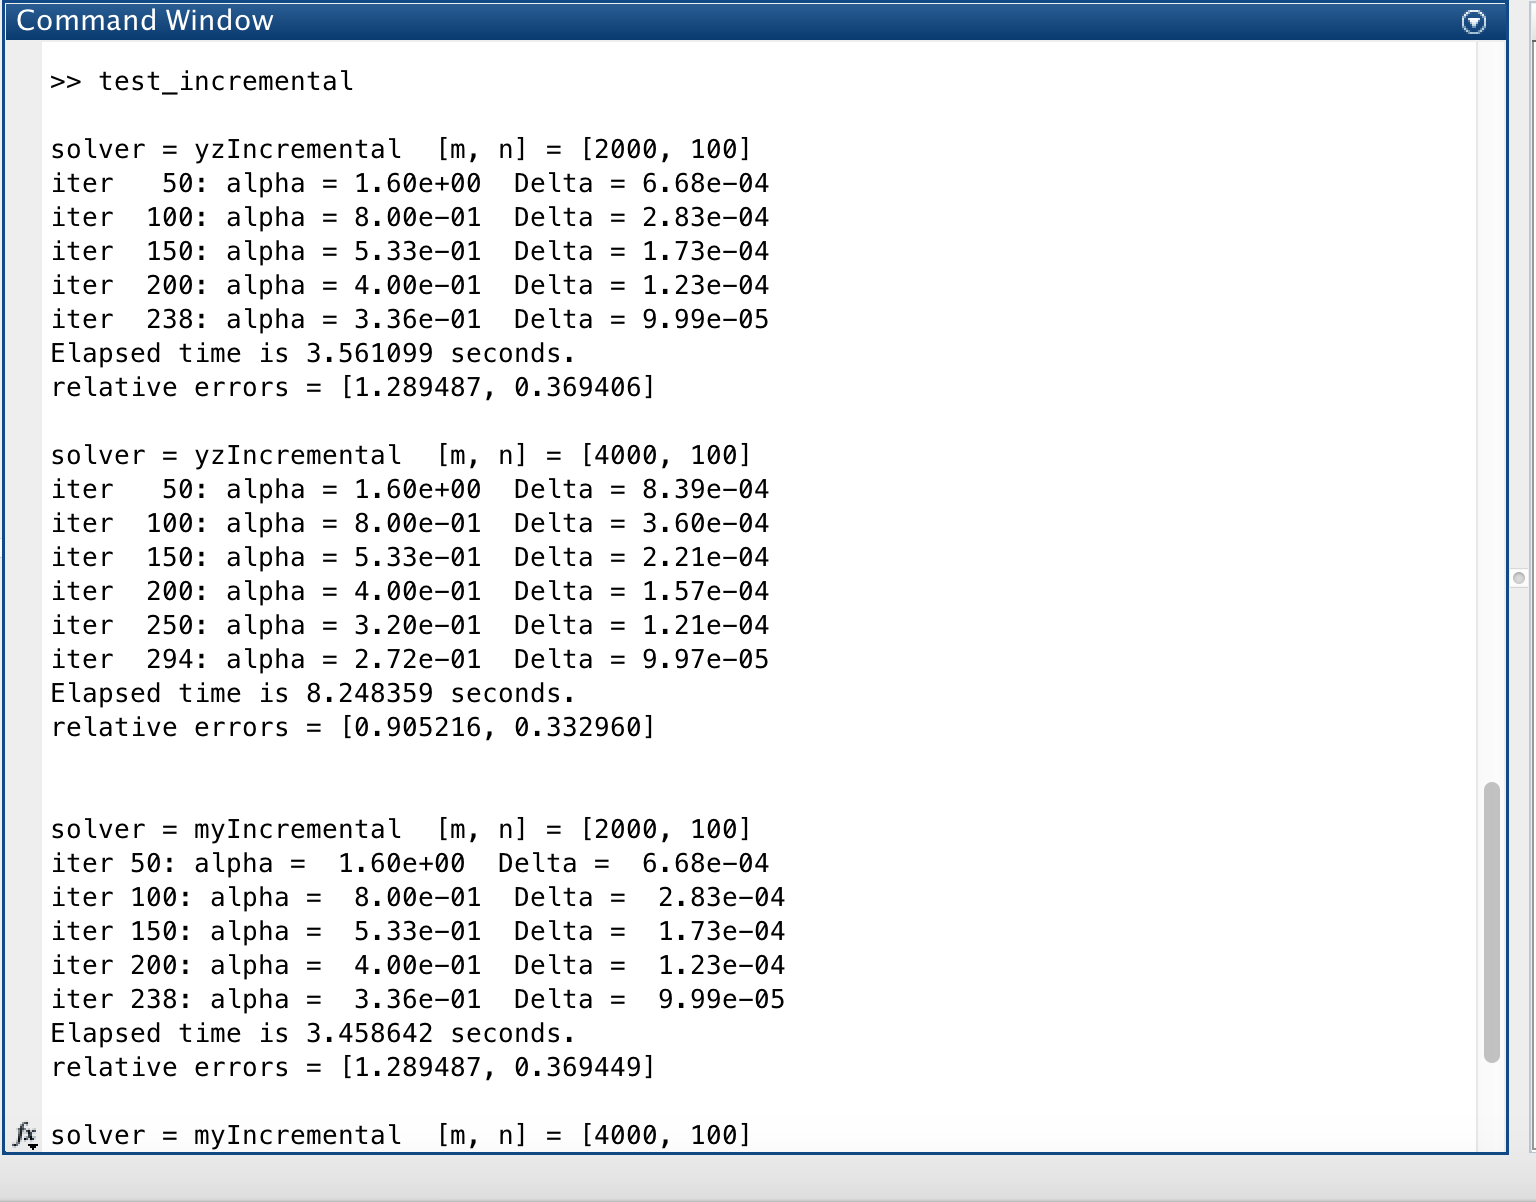
\includegraphics[width=18cm]{f_5}
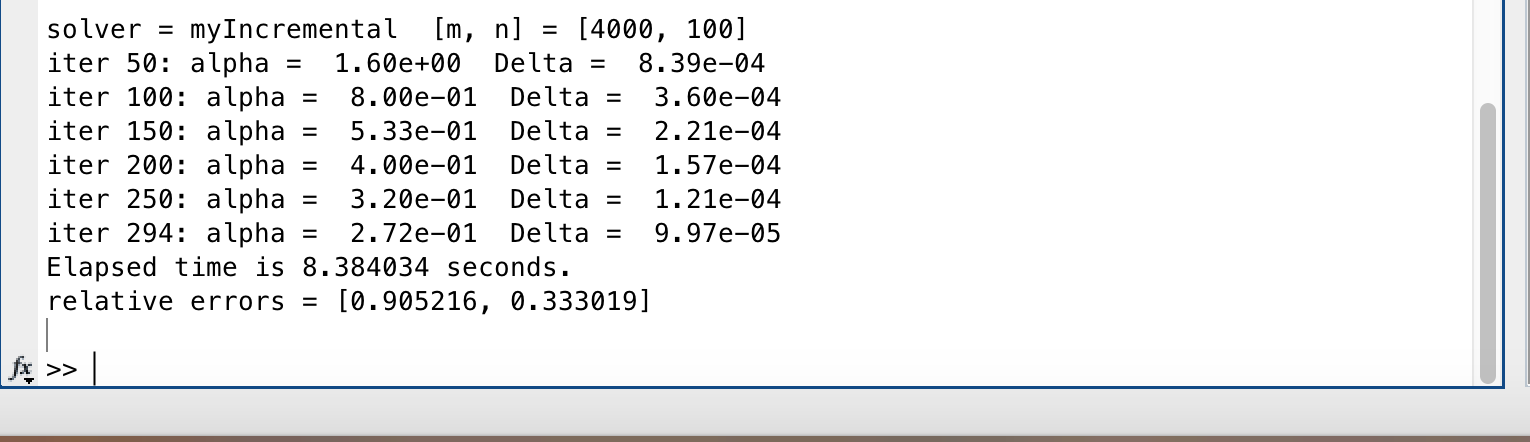
\includegraphics[width=18cm]{f_6}
\caption{Matlab Screen Printout from file test$\_$incremental}
\end{figure}
\subsection*{MATLAB Screen Printout for test incremental2}
\begin{figure}[H]
\centering
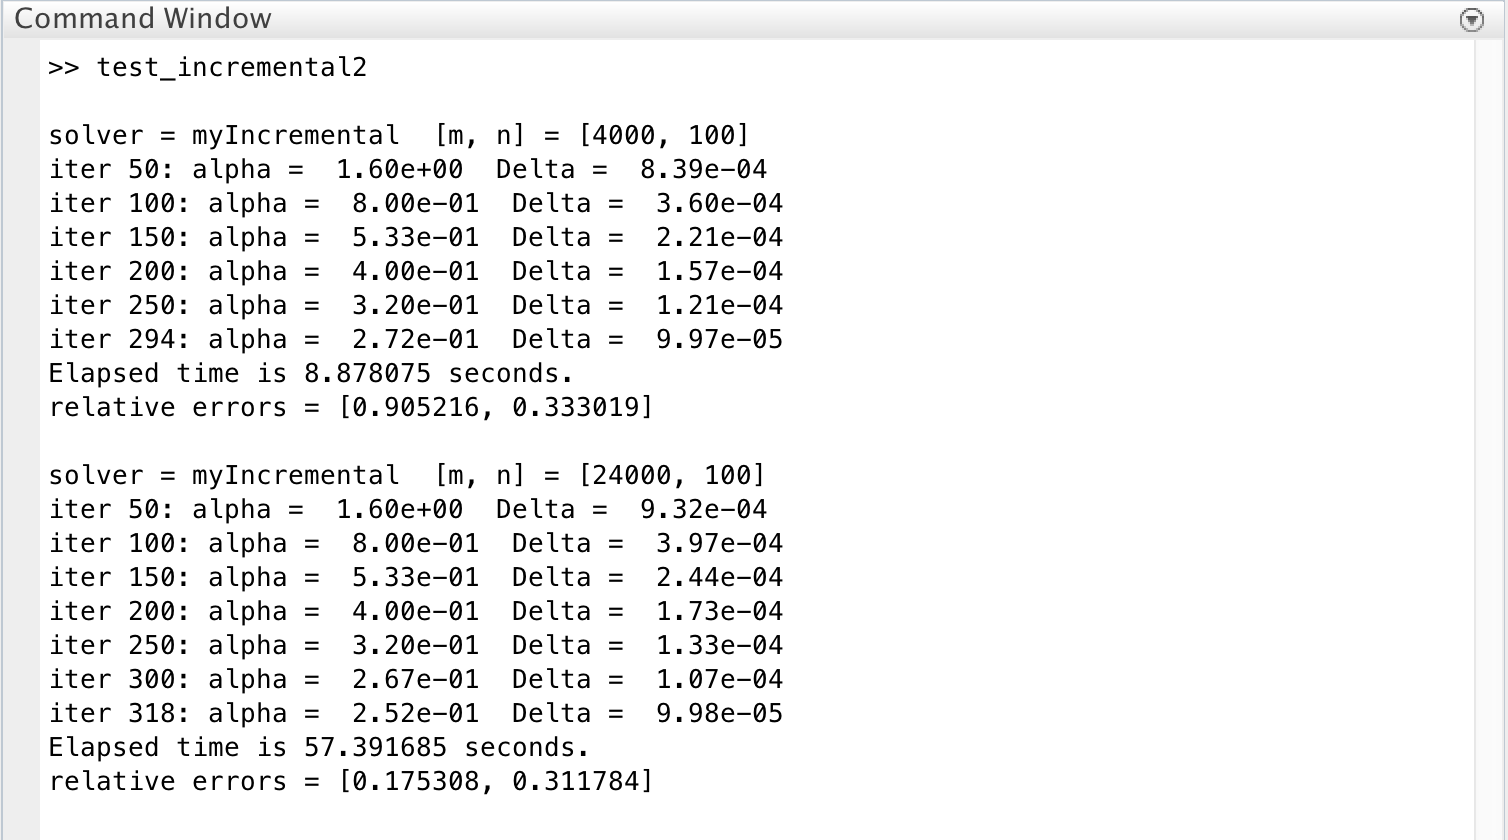
\includegraphics[width=18cm]{f_11}
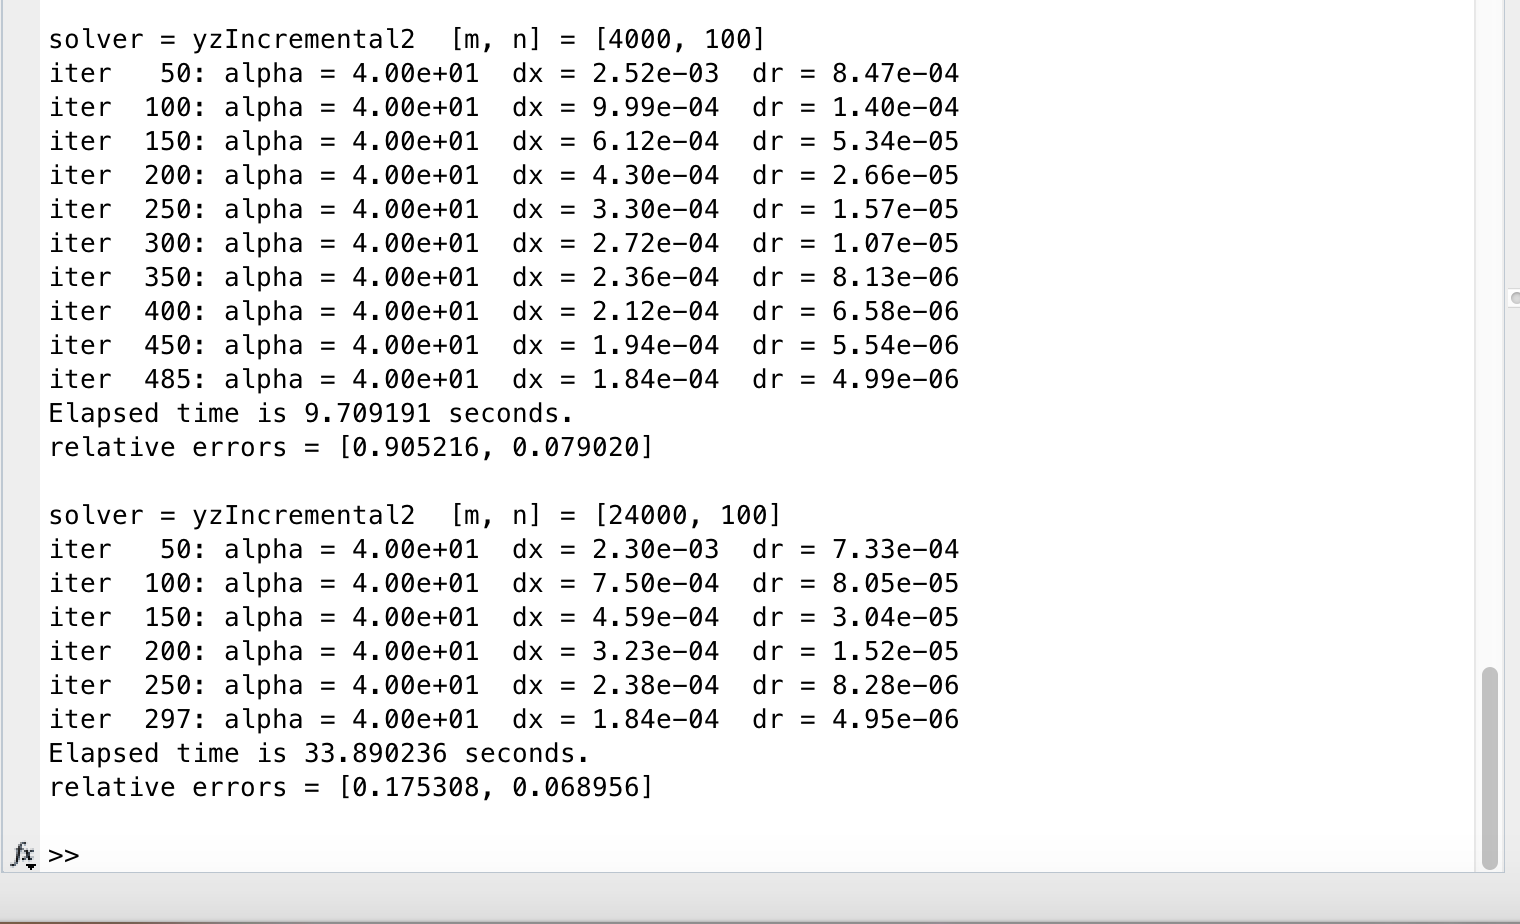
\includegraphics[width=18cm]{f_12}
\caption{Matlab Screen Printout from file test$\_$incremental2}
\end{figure}


\clearpage
\subsection*{Matlab Output figures for test incremental}
\begin{figure}[H]
\centering

\includegraphics[width=12cm]{f_1}
\caption{Matlab Output figures from yzIncremental with$(m,n)=(2000,100)$}
\end{figure}
\begin{figure}[H]
\centering
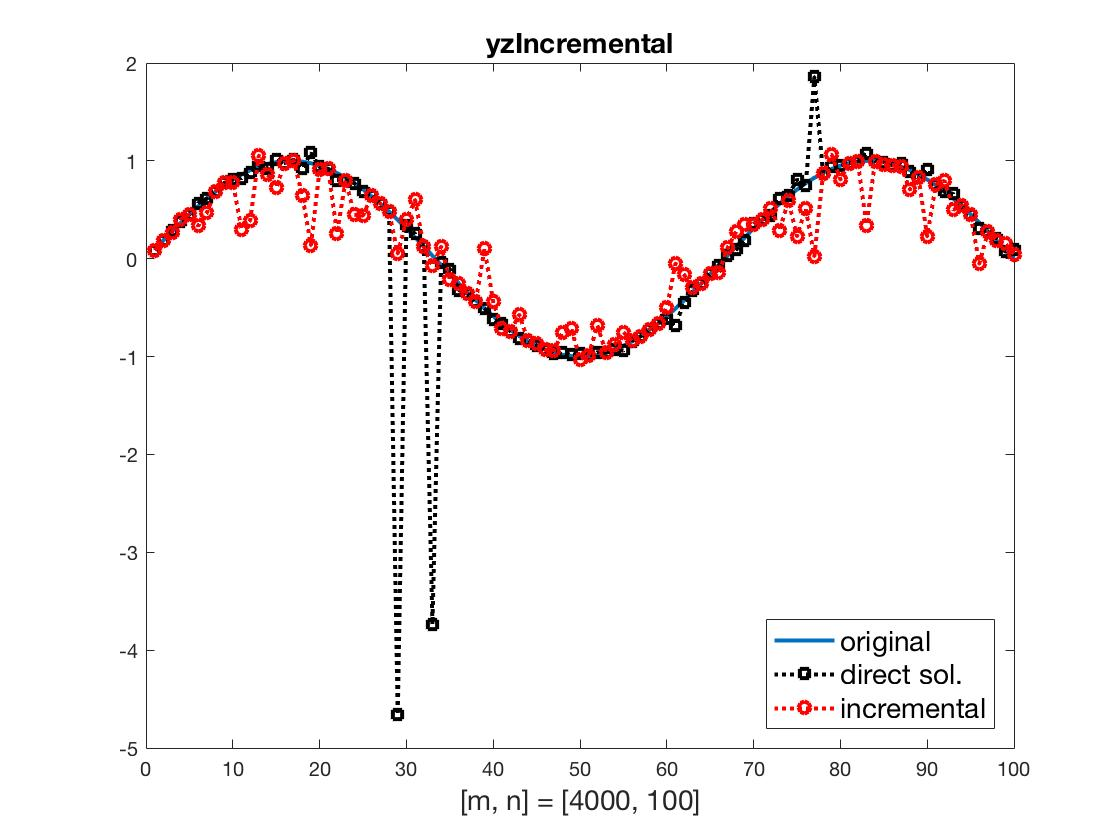
\includegraphics[width=12cm]{f_2}
\caption{Matlab Output figures from yzIncremental with$(m,n)=(4000,100)$}
\end{figure}
\begin{figure}[H]
\centering
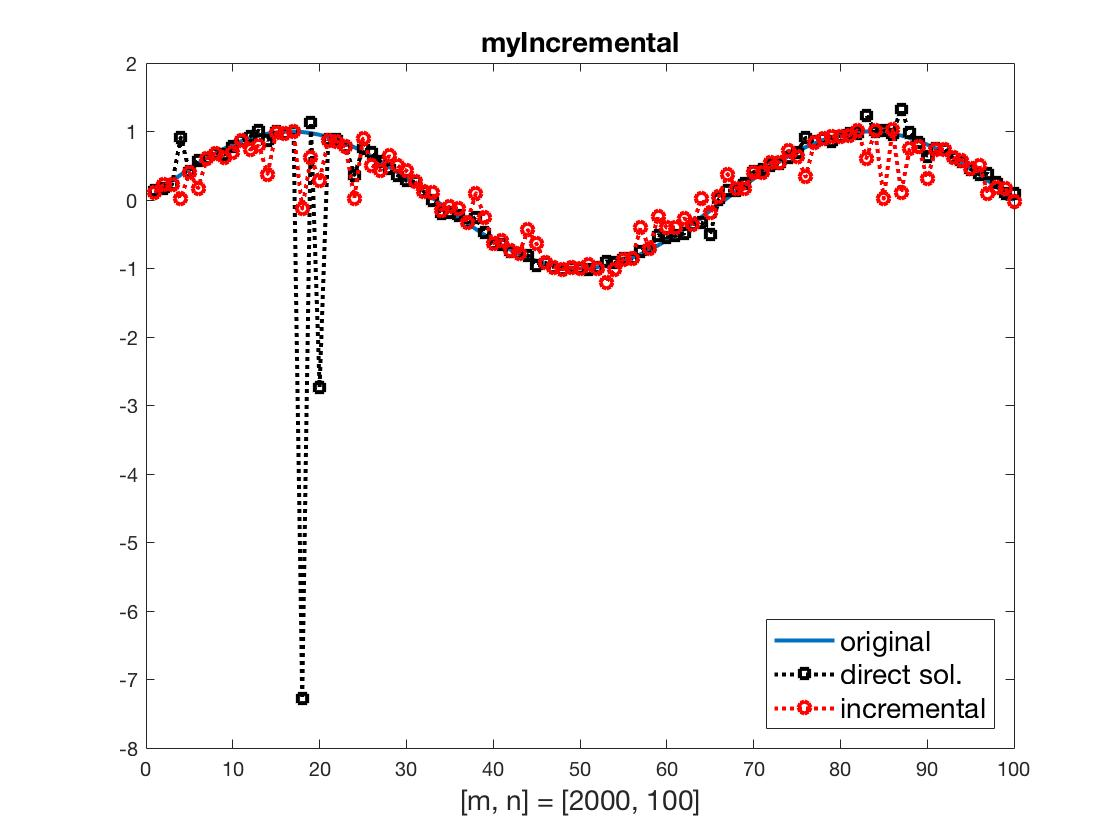
\includegraphics[width=12cm]{f_3}
\caption{Matlab Output figures from myIncremental with$(m,n)=(2000,100)$}
\end{figure}
\begin{figure}[H]
\centering

\includegraphics[width=12cm]{f_4}
\caption{Matlab Output figures from myIncremental with$(m,n)=(4000,100)$}
\end{figure}
\clearpage
\subsection*{Matlab Output figures for test incremental2}
\begin{figure}[H]
\centering
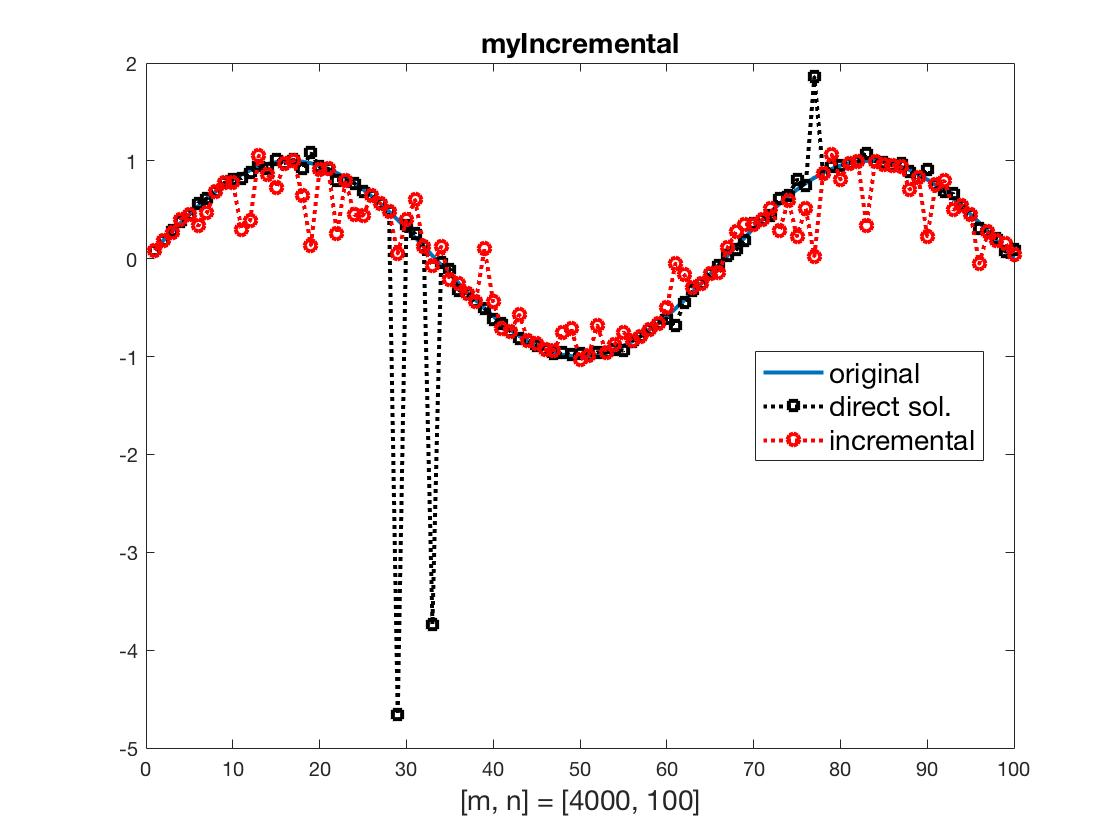
\includegraphics[width=12cm]{f_7}
\caption{Matlab Output figures from myIncremental with$(m,n)=(4000,100)$}
\end{figure}
\begin{figure}[H]
\centering
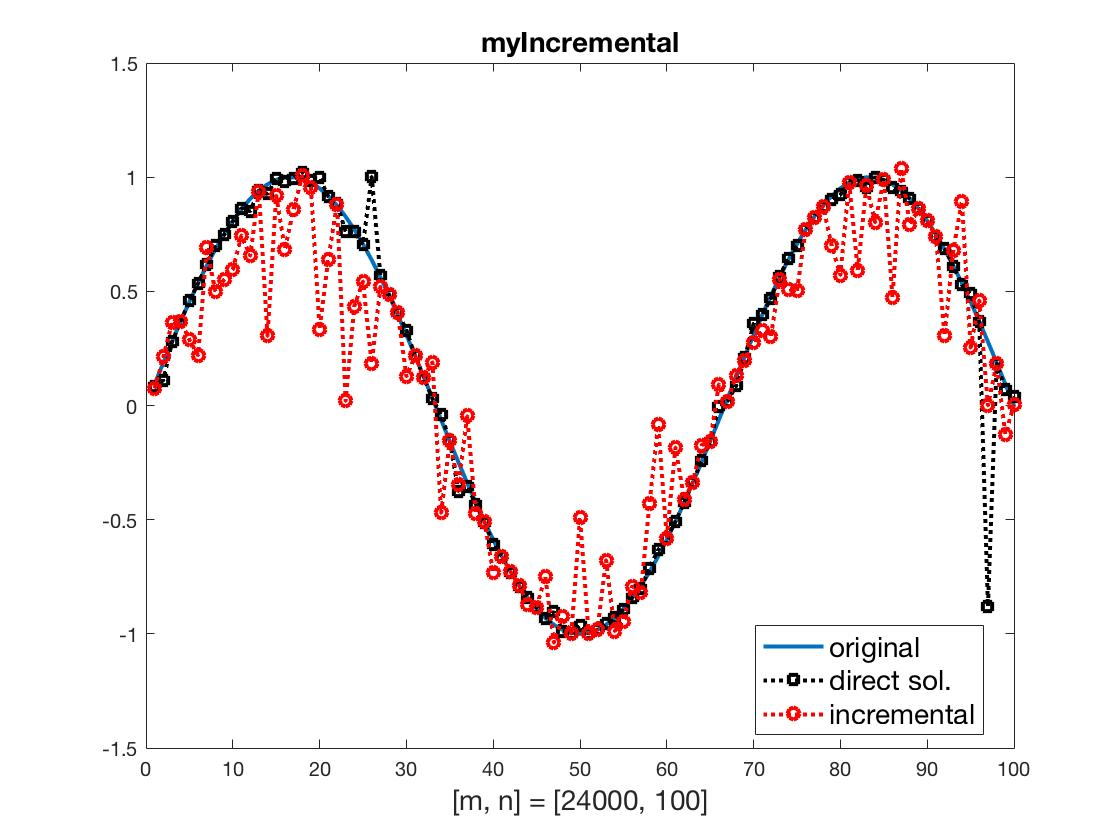
\includegraphics[width=12cm]{f_8}
\caption{Matlab Output figures from myIncremental with$(m,n)=(24000,100)$}
\end{figure}
\begin{figure}[H]
\centering
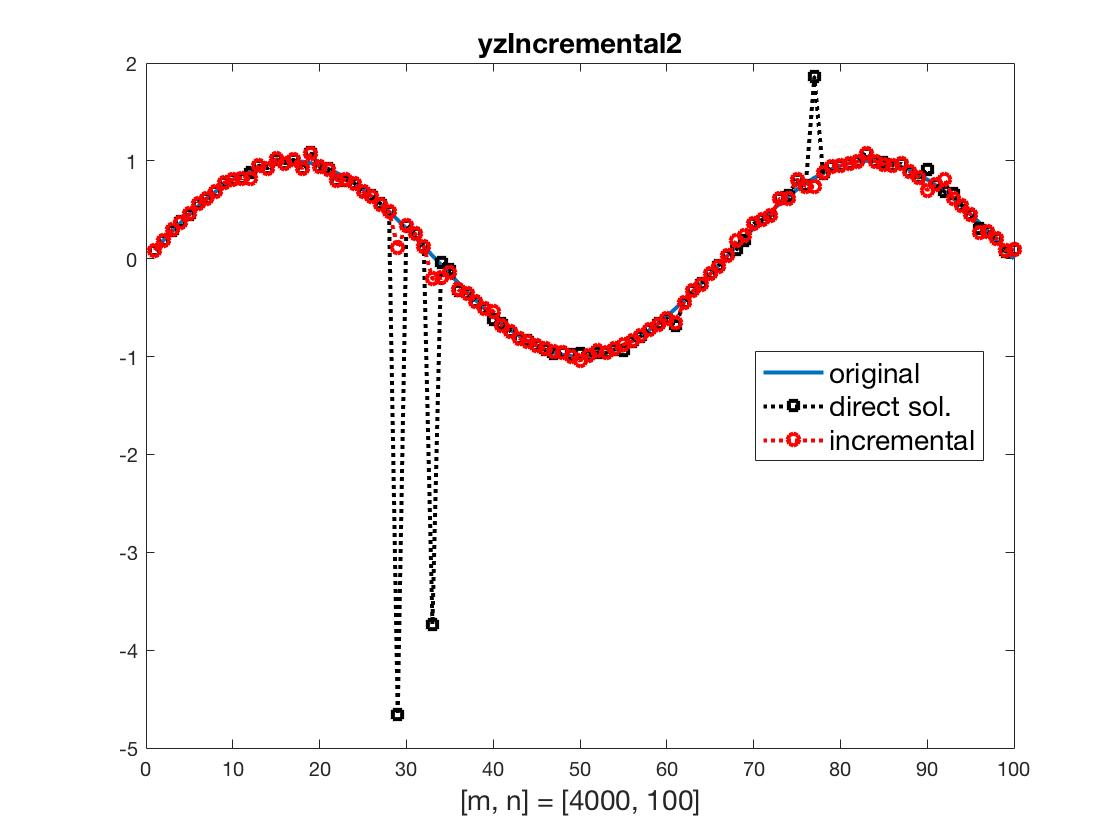
\includegraphics[width=12cm]{f_9}
\caption{Matlab Output figures from yzIncremental2 with$(m,n)=(4000,100)$}
\end{figure}
\begin{figure}[H]
\centering
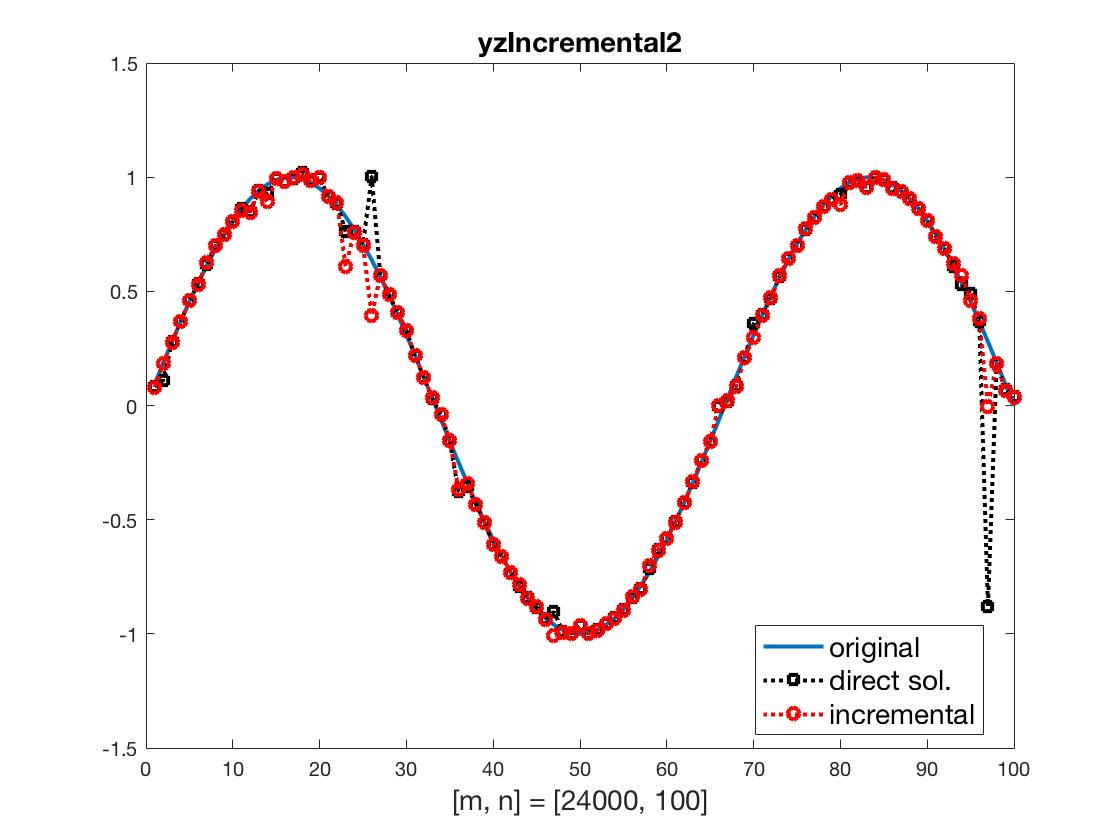
\includegraphics[width=12cm]{f_10}
\caption{Matlab Output figures from yzIncremental2 with$(m,n)=(24000,100)$}
\end{figure}
\clearpage
\subsection*{Short Summary}
\paragraph{Introduction}
This project aims to solve the least squares problem by taking descent directions on each sub-functions iteratively in each iteration.
\paragraph{Save necessity before computation}
In each iteration we are required to update our $\bm x$ with 
\[
\bm x\leftarrow\bm x-\alpha*\nabla f_i(x)=\bm x-\alpha*(a_i*(a_i\trans x-b_i))
\] 
for many times, which is expansive since MATLAB spends lots of time calling rows of large matrix $\bm A$. However, if we pre-save the rows of $\bm A$ and write a function handle to replace the update command, the code will run much faster.
\paragraph{Choose Reasonable parameters}
For example, the dimishing step-size should be relatively large when starting the update, so if choosing tiny step size in the beginning, it is difficult for the code to converge.
\paragraph{Comments about yzincremental2}
In the new file yzincremental2, Prof. YZ apply the constant step size, but the results are better compared with that by applying dimishing step size. As he said in the lecture, the insights and reasons behind this is still remained to be found.










\clearpage
\section*{MATLAB Project: Primal-dual interior-point method for LP}
\subsection*{A copy of my code: my pdipm.m(predictor-corrector algorithm)}
\begin{lstlisting}[language=matlab]
function [x,y,z,iter] = my_pdipm(A,b,c,tol,maxit,prt)
% Input:
%           A = constraint coefficient matrix
%           b = constraint right-hand side vector
%           c = objective coefficient vector
%         tol = tolerance
%       maxit = maximum number of iterations allowed
%         prt = switch for screen printout (1 on, 0 off)
% Output:
%           x = computed primal solution
%           y = computed dual solution
%           z = computed dual slacks
%        iter = iteration counter
%% parameters setting
%p = symamd(abs(A)*abs(A)');     
[m,n]=size(A);
p = symamd(abs(A)*abs(A)');%colamd(A');%symamd(A*A');%colamd(A');
%% Initialize
bigMfac = 100;
bigM = max(max(abs(A)));
bigM = max([norm(b,Inf), norm(c,Inf), bigM]);
x = bigMfac*bigM * ones(n,1); %bigMfac*bigM * ones(n,1);    
y = zeros(m,1);     
z = x;
%bc = 1 + max(norm(b),norm(c));
bc = 1+[norm(b);norm(c);0];
for iter = 1:maxit
    %% initial setting
    rd = -c + A'*y + z;
    rp = -b + A*x;
    rc = x.*z;
    gap = mean(rc);
    %% Stopping criteria
    bc(3) = abs(b'*y)+1;
    residual = sum([norm(rp);norm(rd);norm(rc)]./bc);
    if residual <= tol, break;end;
    switch prt
        case 1
            fprintf('iter %2i: [primal dual gap] = [%9.2e  %9.2e  %9.2e]\n',iter,[norm(rp);norm(rd);norm(rc)]./bc);
    end
    %% formulate the linear systems
    d = min(5.e+15,x./z);
    M = A* sparse(1:n,1:n,d) *A';   R = chol(M(p,p));%R = chol(M(p,p),'lower','vector');
    %% Predictor step: Solve for dy
    t1 = x.*rd - rc;
    t2 = -(rp+A*(t1./z));
    dy1 = zeros(m,1);
    dy1(p) = R\(R'\t2(p));
    %% Predictor step: Solve for dz, dx by back substitutions
    dx1 = (t1 + x.*(A'*dy1))./z;
    dz1 = (-rc - z.* dx1)./x;
    %% Corrector Step
    ap = -1/min(min(dx1./x),-1);
    ad = -1/min(min(dz1./z),-1);
    % centering parameter step
    mun = ((x + ap * dx1)' * (z + ap * dz1))/n;
    sigma = (mun/gap)^3;
    mu = gap * min(.2,sigma);
    rd = 0; rp = 0; rc = -mu + dx1.*dz1;
    t1 = x.*rd - rc;
    t2 = -(rp+A*(t1./z));
    dy2 = zeros(m,1);
    dy2(p) = R\(R'\t2(p));
    dx2 = (t1 + x.*(A'*dy2))./z;
    dz2 = (-rc - z.* dx2)./x;
    %% Combined Step
    dx = dx1+dx2;   dy = dy1 + dy2; dz = dz1+dz2;
    tau = max(.9995,1-10*gap);
    ap = -1/min(min(dx./x),-1);
    ad = -1/min(min(dz./z),-1);
    ap = min(tau * ap,1);
    ad = min(tau * ad,1);
    x = x + ap * dx;
    z = z + ad * dz;
    y = y + ad * dy;
end
x=full(x); z=full(z); y=full(y);
end
\end{lstlisting}

\subsection*{A copy of my code: my pdip.m (basic algorithm)}
\begin{lstlisting}[language=matlab]
function [x,y,z,iter] = my_pdipm(A,b,c,tol,maxit,prt)
% Input:
%           A = constraint coefficient matrix
%           b = constraint right-hand side vector
%           c = objective coefficient vector
%         tol = tolerance
%       maxit = maximum number of iterations allowed
%         prt = switch for screen printout (1 on, 0 off)
% Output:
%           x = computed primal solution
%           y = computed dual solution
%           z = computed dual slacks
%        iter = iteration counter


%% parameters setting
%p = symamd(abs(A)*abs(A)');     
[m,n]=size(A);
p = colamd(A');%symamd(A*A');%colamd(A');
%% Initialize
bigMfac = 100;
bigM = max(max(abs(A)));
bigM = max([norm(b,Inf), norm(c,Inf), bigM]);
x = bigMfac*bigM * ones(n,1);    
y = zeros(m,1);     
z = x;
%bc = 1 + max(norm(b),norm(c));
bc = 1+[norm(b);norm(c);0];
for iter = 1:maxit
    %% initial setting
    rd = -c + A'*y + z;
    rp = -b + A*x;
    rc = x.*z;
    %% Stopping criteria
    bc(3) = abs(b'*y)+1;
    residual = sum([norm(rp);norm(rd);norm(rc)]./bc);
    if residual <= tol, break;end;
    switch prt
        case 1
            fprintf('iter %2i: [primal dual gap] = [%9.2e  %9.2e  %9.2e]\n',iter,norm([rd;rp;rc])./bc);
    end
    %% Update rc
    gap = mean(rc);
    rc = rc - min(.1,100*gap)*gap;
    %% Solving for dy
    d = min(5.e+15,x./z);
    M = A* sparse(1:n,1:n,d) *A';   R = chol(M(p,p));%R = chol(M(p,p),'lower','vector');
    t1 = x.*rd - rc;
    t2 = -(rp+A*(t1./z));
    dy = zeros(m,1);
    dy(p) = R\(R'\t2(p));
    %% Solving for dz, dx by back substitutions
    dx = (t1 + x.*(A'*dy))./z;
    dz = (-rc - z.* dx)./x;
    %% Determine the primal and dual step sizes
    tau = max(.9995,1-gap);
    ap = -1/min(min(dx./x),-1);
    ad = -1/min(min(dz./z),-1);
    ap = min(tau * ap,1);
    ad = min(tau * ad,1);
    x = x + ap * dx;
    z = z + ad * dz;
    y = y + ad * dy;
end
x=full(x); z=full(z); y=full(y);
end
\end{lstlisting}
\clearpage
\subsection*{MATLAB Screen printout for the run results of test$\_$ipm1.m with $r=4$}
\begin{figure}[H]
\centering
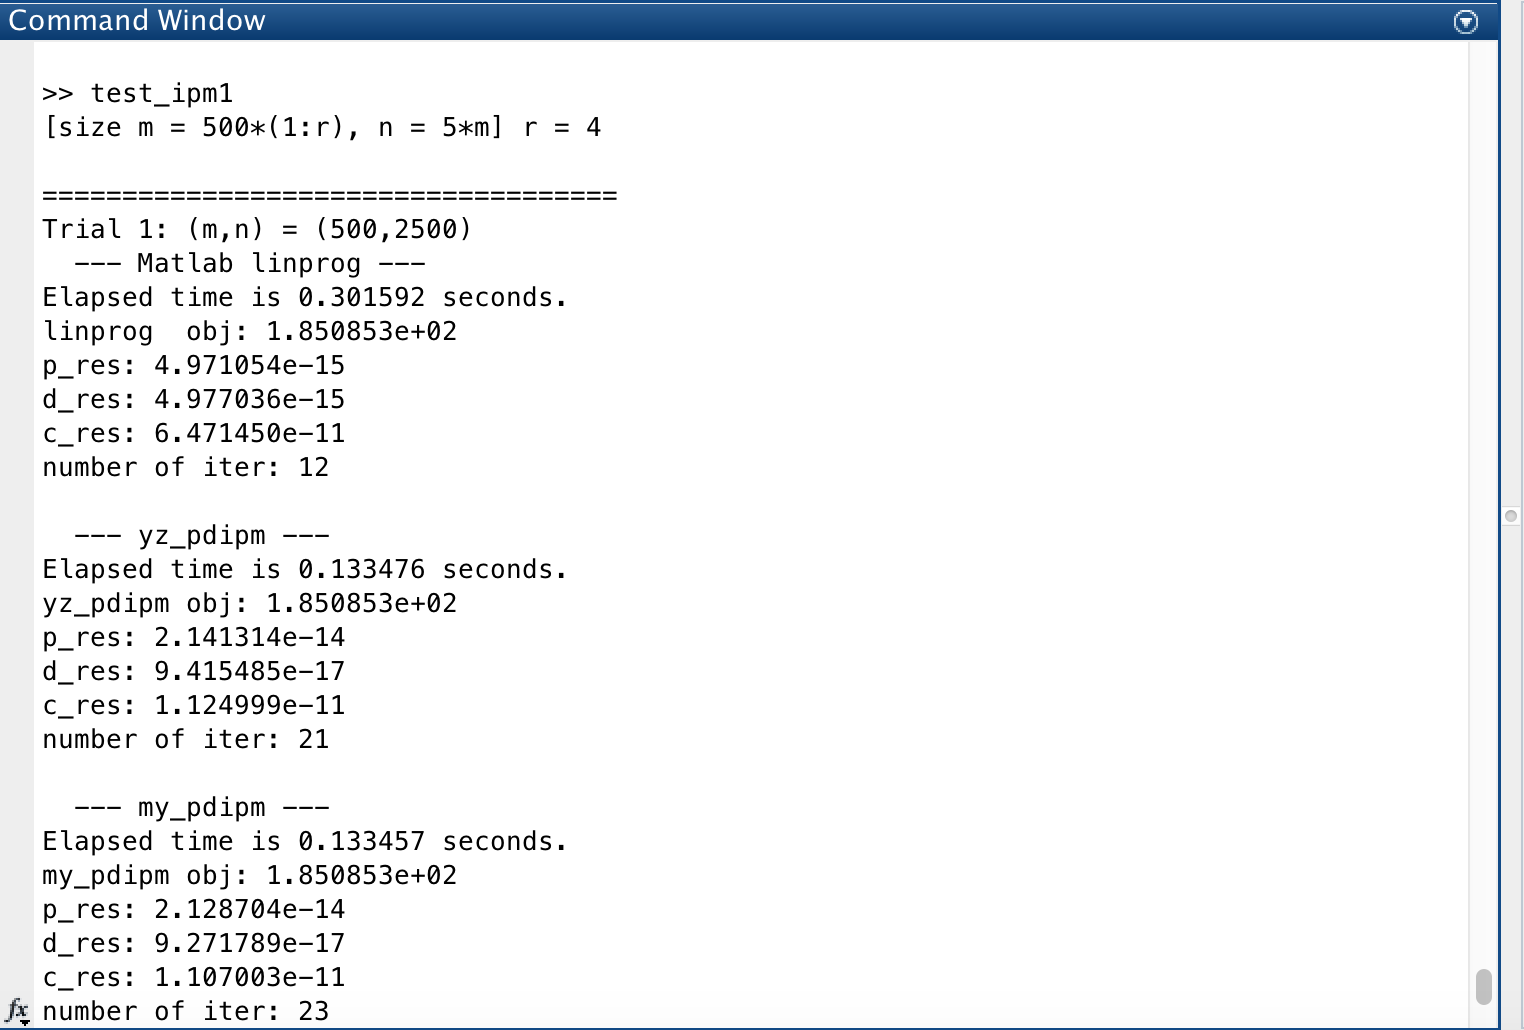
\includegraphics[width=15cm]{f_13}
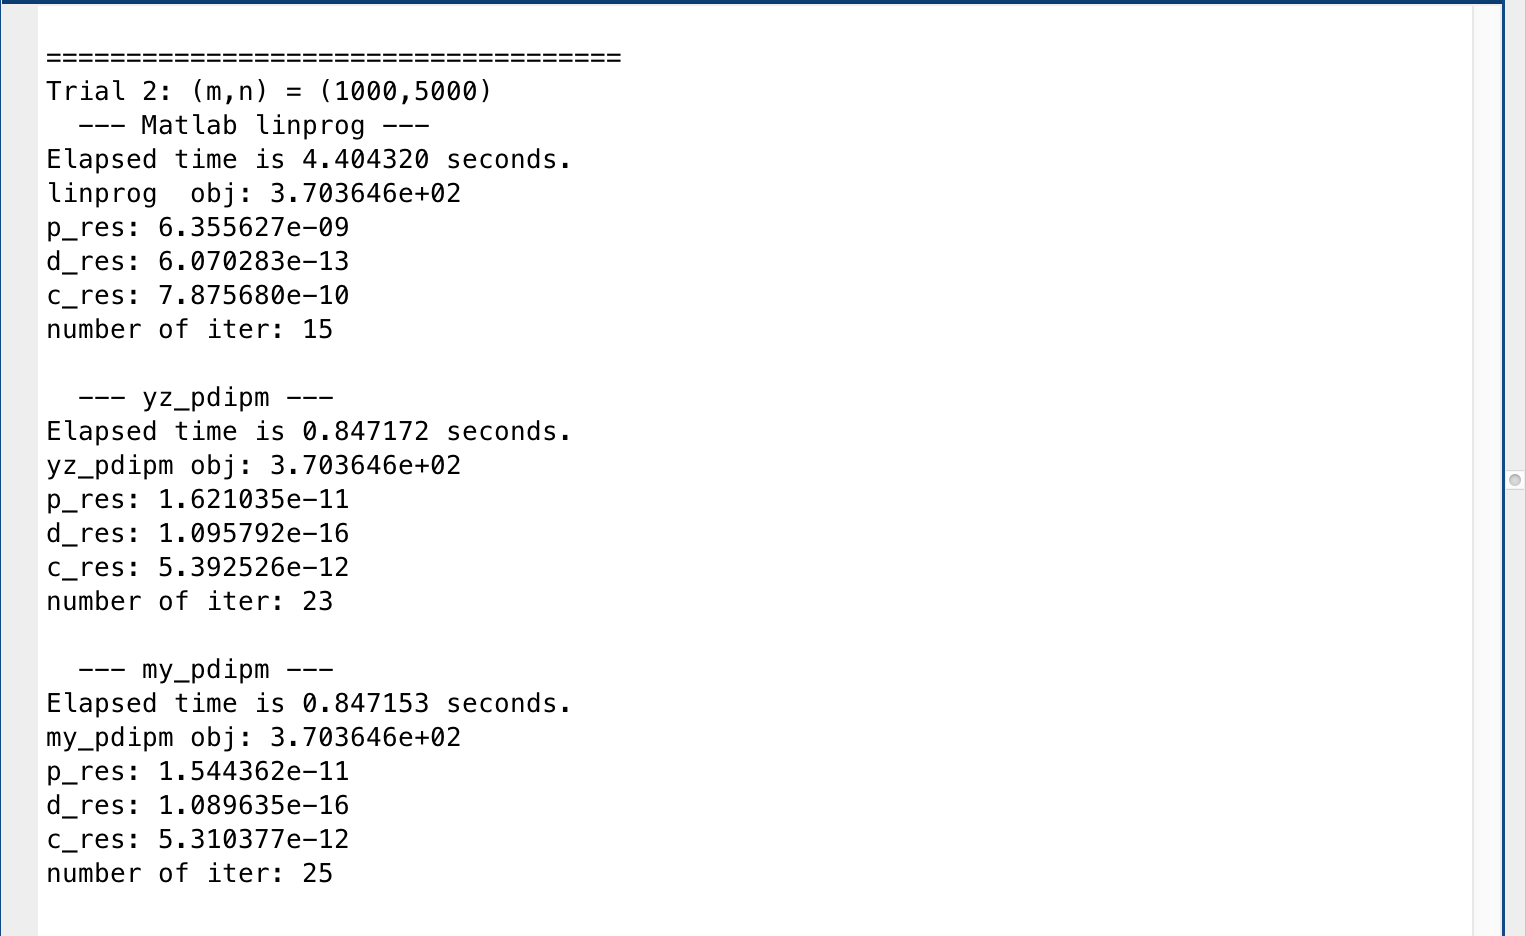
\includegraphics[width=15cm]{f_14}
\caption{Matlab Screen Printout from file test$\_$ipm1.m with $r=4$}
\end{figure}
\begin{figure}[H]
\centering
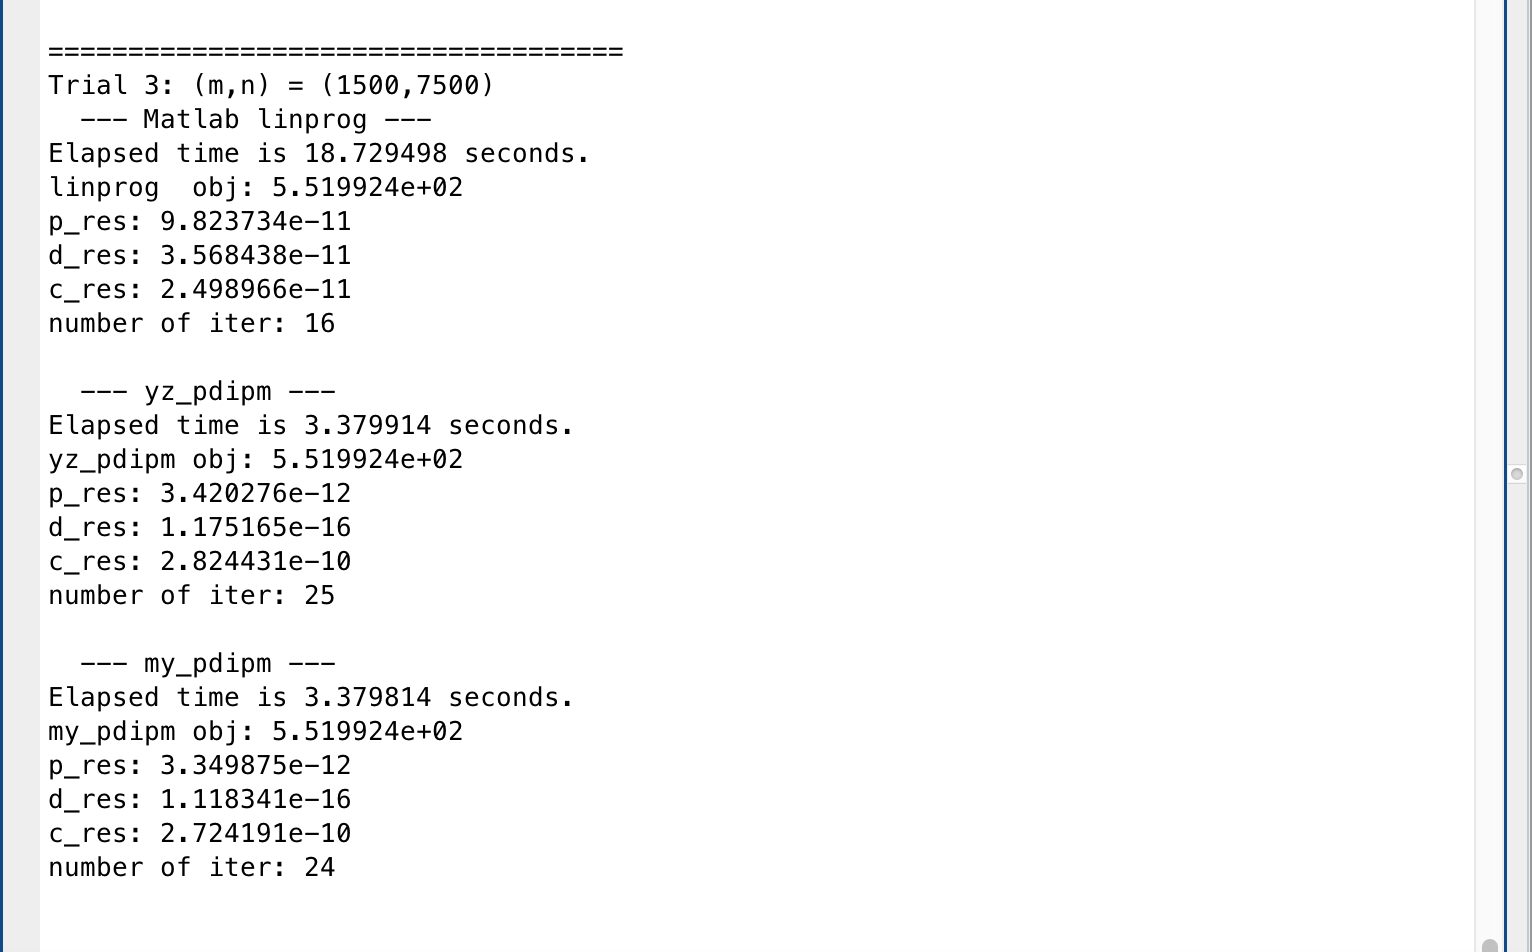
\includegraphics[width=15cm]{f_15}
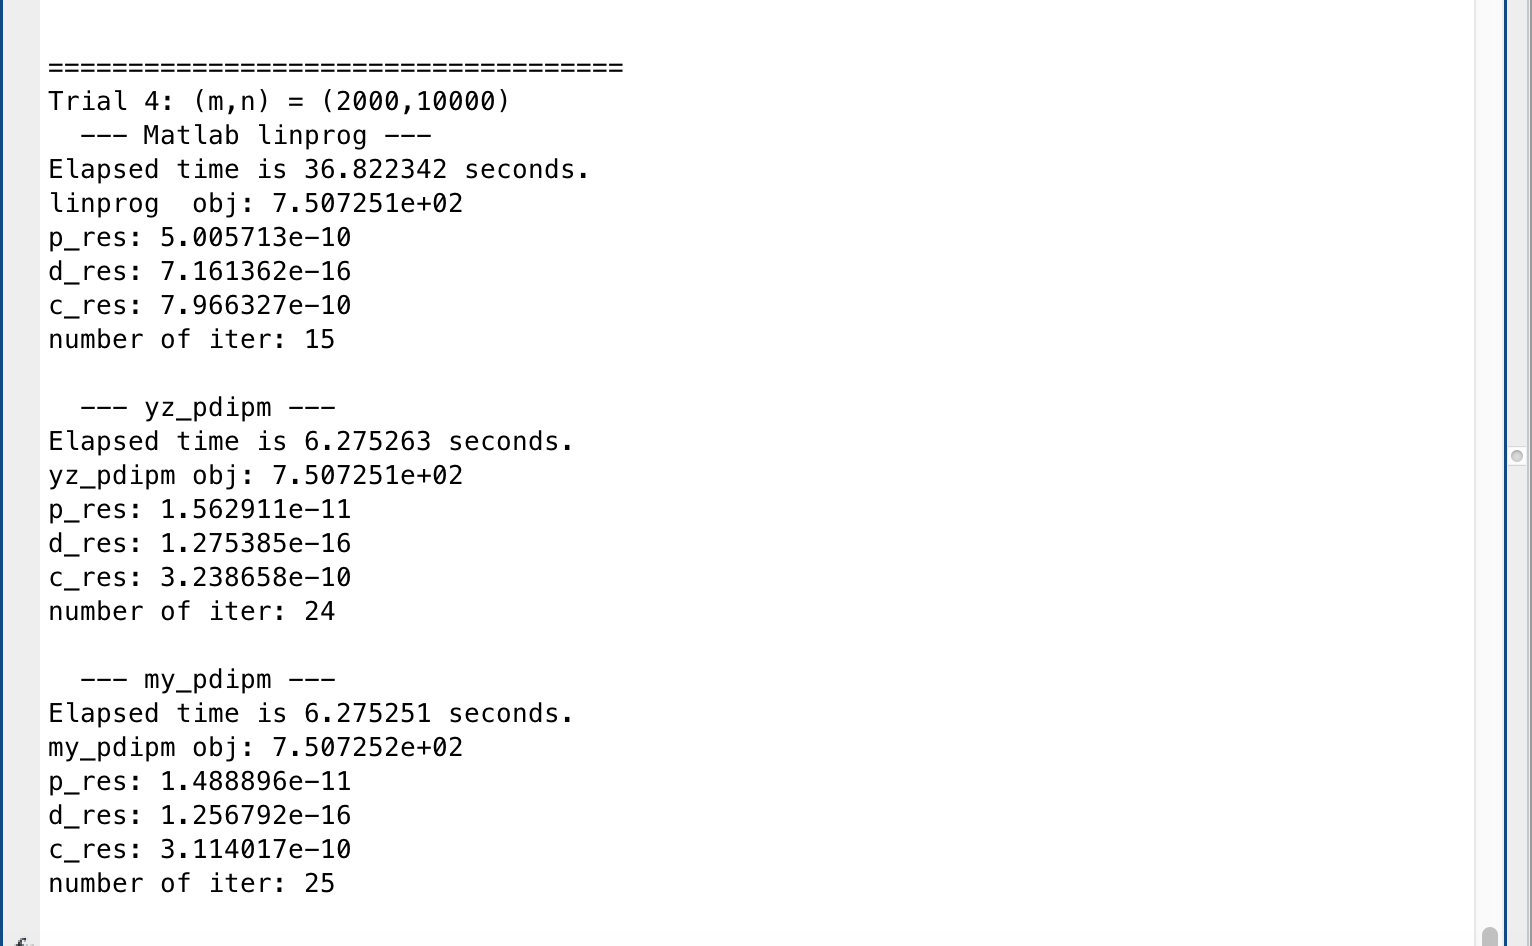
\includegraphics[width=15cm]{f_16}
\caption{Matlab Screen Printout from file test$\_$ipm1.m with $r=4$}
\end{figure}
\begin{figure}[H]
\centering
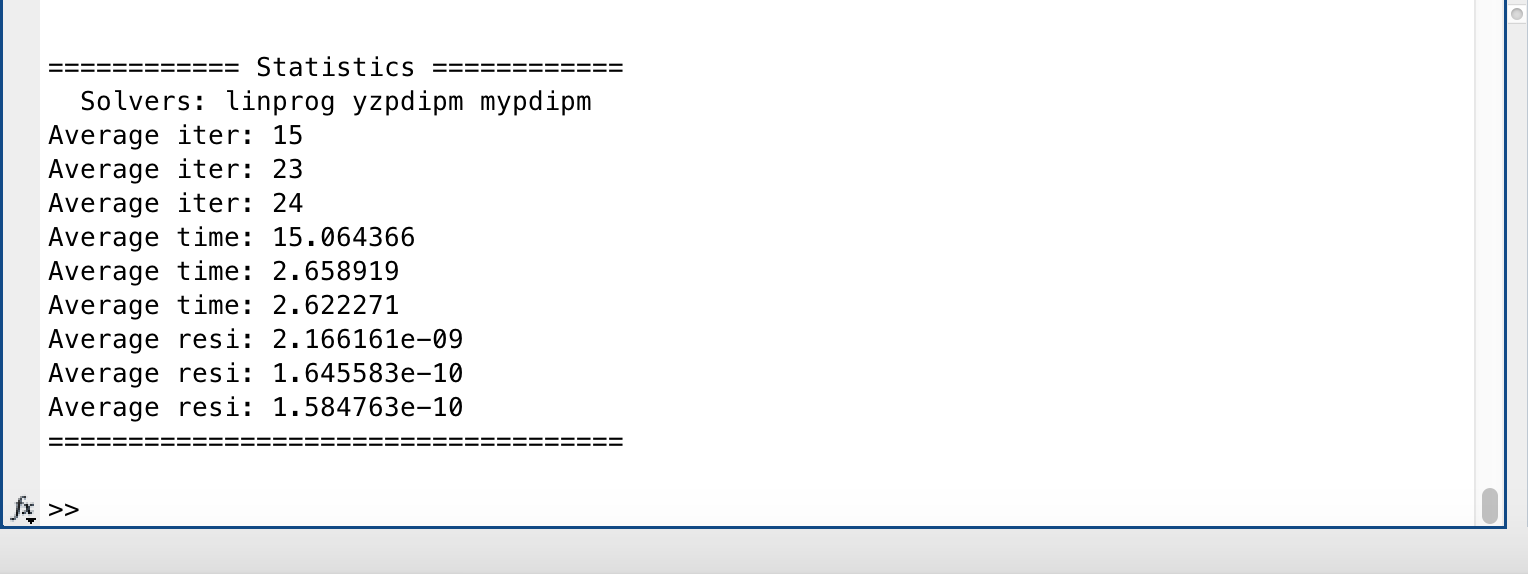
\includegraphics[width=15cm]{f_17}
\caption{Matlab Screen Printout from file test$\_$ipm1.m with $r=4$}
\end{figure}
\subsection*{MATLAB Screen printout for the run results of test$\_$ipm2.m}
\begin{figure}[H]
\centering
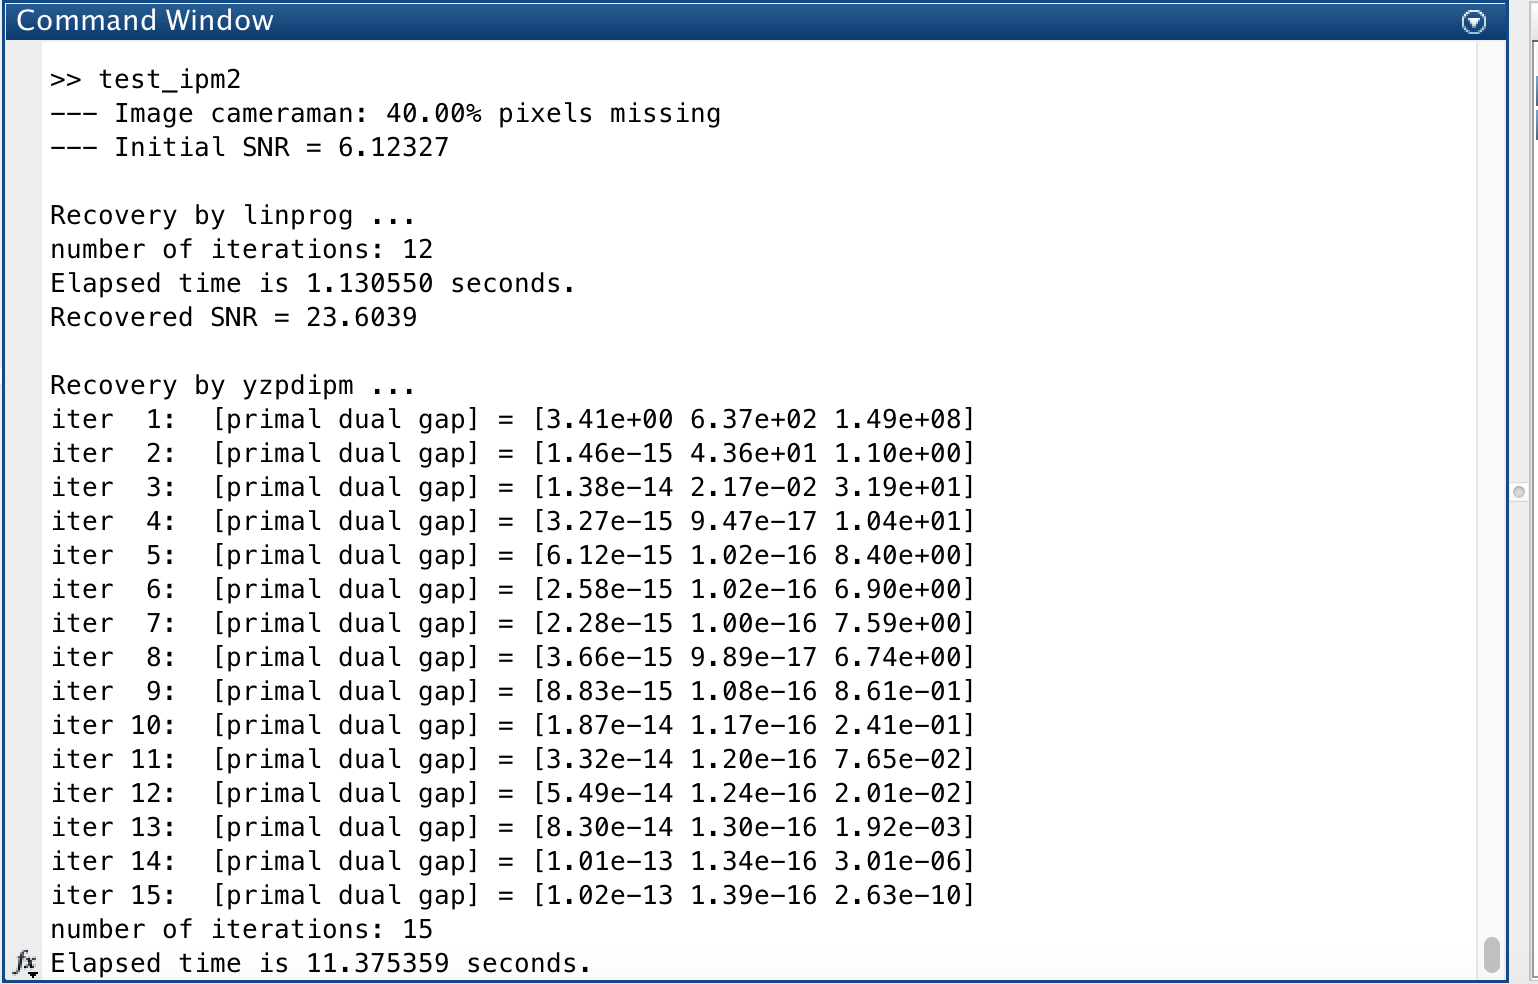
\includegraphics[width=15cm]{f_18}
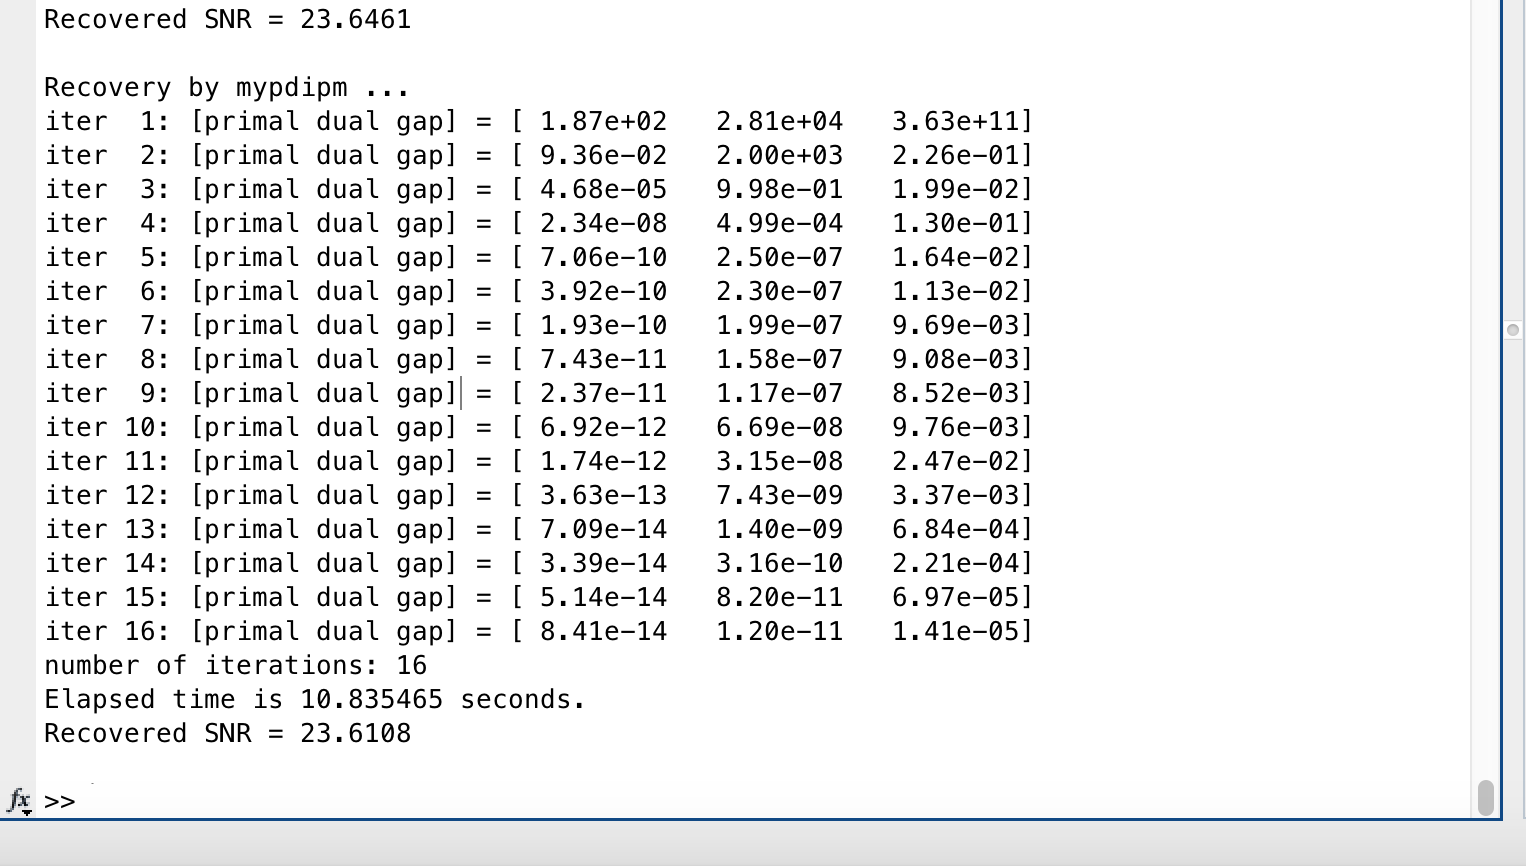
\includegraphics[width=15cm]{f_19}
\caption{Matlab Screen Printout from file test$\_$ipm2.m}
\end{figure}
\clearpage
\subsection*{MATLAB Output Figures}
\begin{figure}[H]
\centering
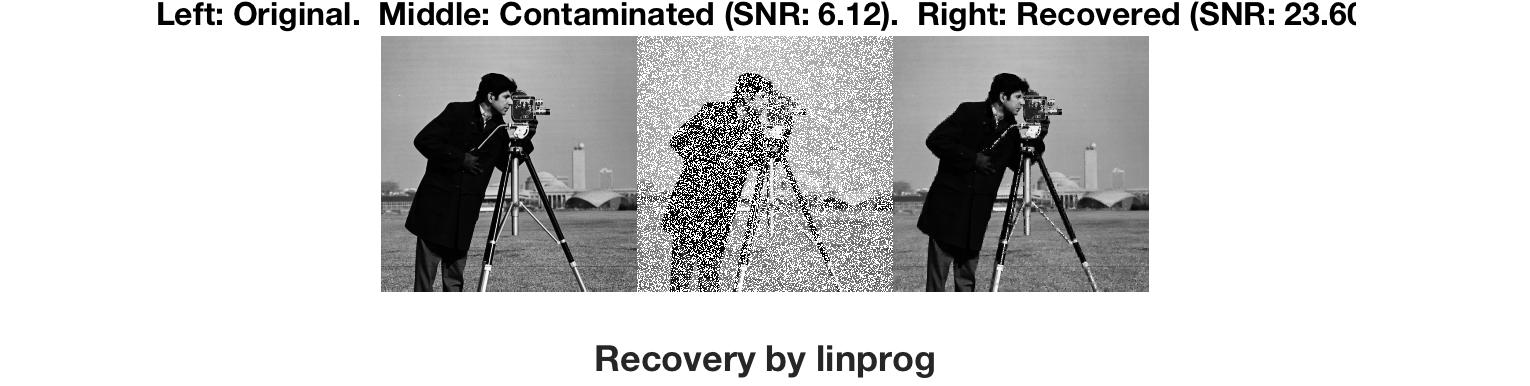
\includegraphics[width=19cm]{f_2_1}
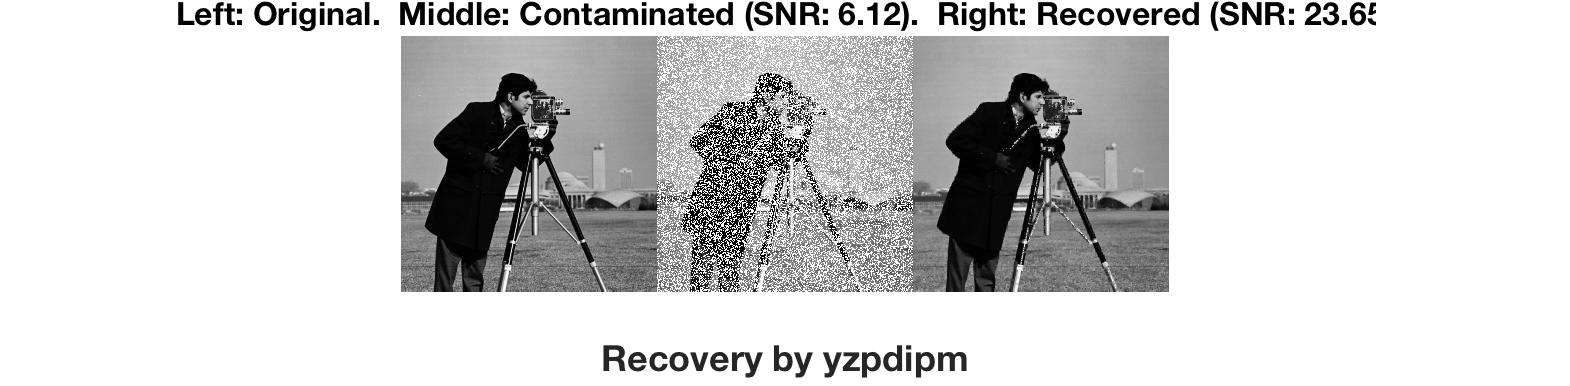
\includegraphics[width=19cm]{f_2_2}
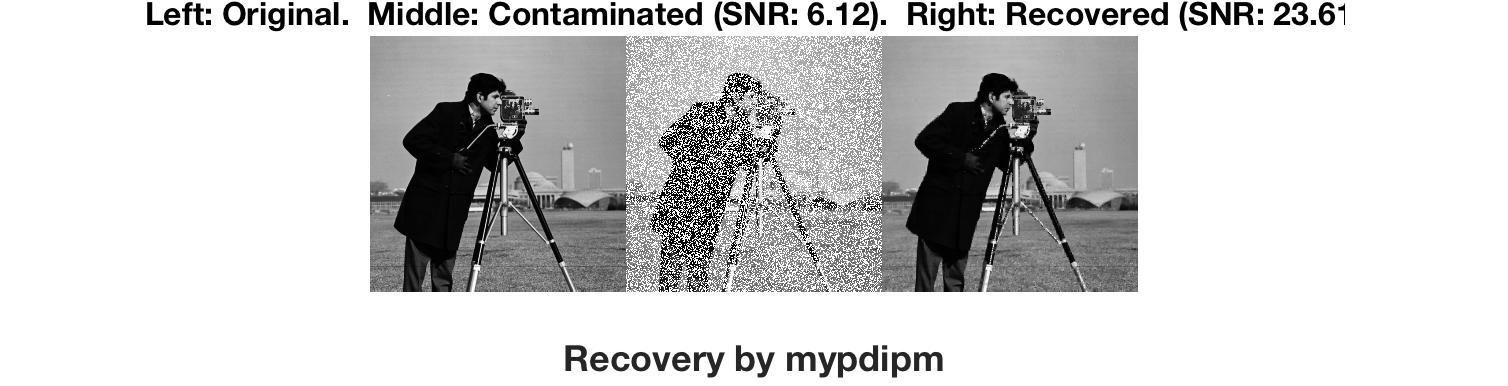
\includegraphics[width=19cm]{f_2_3}
\caption{Matlab Output figures from file test$\_$ipm2.m}
\end{figure}

\clearpage
\subsection*{Short Summary}
\paragraph{Introduction}
This project aims to apply primal-dual interior point method to sovle linear programming. The basic idea is to solve the primal and dual simultaneously, i.e., keep the primal feasiblity and dual feasibility, and try to achieve the complementary condition with iteration going on.
\paragraph{Performance summary}
This algorithm has fast convergence rate in general. As shown in the MATLAB screen printout, the gap between primal and dual optimal solution decreases with order $O(n^{3.5})$.
\paragraph{Care about initial guess}Do care about initial guess of feasble solution of LP, otherwise with the iteration going on,  you may find the computer cannot compute the Cholesky factorization. One relatively good initial guess is $100\times\max\{A_i\}*\bm1$ for the specific LP satisfying the equality constraint $(\bm{Ax})_i=\sum_jA_{ij}$
\paragraph{Save the necessity before computation}
For example, we need to use the values for $-x.*rd+rc$ for many times, so we can save it in advance and call them if necessary; moreover, saving the matrix $\diag(x_1/z_1,\dots,x_n/z_n)$ is meaningless, since we can arrange computation such that it suffices to save the vector form $x./z$ instead.
\paragraph{Appreciate the sparse form and Cholesky factorization}
The Cholesky factorization gives us an alternative to obtain an inverse of a large sparse matrix $\bm A$, otherwise in each iteration we need to compute the matrix inverse inefficiently. Also, if order the columns of $\bm A$ appropriately by using command $p=colamd(\bm A)$ and $chol(\bm A(p,p))$, the computation will be much more easier.
\paragraph{Appreciate Predictor-Corrector Algorithm}
\begin{itemize}
\item
Introduction: The preidction step aims to \emph{extrapolate} the optimal value of the next iteration, i.e., calculate an initial guess of the best output for next iteration; the corrector step aims to improve the initial guess using some rules such as \emph{trapezodial rule}. Such an algorithm is useful in solving differential equation, but recently we find that it is also useful for optimization problem.
\item
Advantage: By applying this method, we can solve the linear system in a more efficient and accurate way than the old algorithm. In particular, the disadvantage for the older one is that sometimes the linear system is singular, which makes the computer unable to continue the computation. However, this algorithm can solve the linear system correctly, which crosses over this obstacle.
\end{itemize} 













\end{document}